\chapter{A1 External resources}\label{External resources}
We refer the reader to the following resources online, which have not been included in this report, due to limited space:
\begin{itemize}
\item A demonstration of the expected Robot Programming by Demonstration process using our proposed framework: \url{https://youtu.be/I6m_0lpI_ZM}
\item GitHub repository: \url{https://github.com/ysl208/Baxter_PbD/tree/master}
\end{itemize}
\chapter{A2 PDDL code}\label{PRODUCTION domain}
\section{PRODUCTION planning domain}
\begin{verbatim}
(define (domain PRODUCTION)
   (:requirements :typing)
   (:types zone table - location
           metal wood - product)
   (:constants right - gripper)
   (:predicates (at-gripper ?g - gripper ?l - location)
                (at ?p - product ?l - location)
                (free ?g - gripper)
                (empty ?l - location)
                (carry ?p - product ?g - gripper))

(:action pick
    :parameters (?p - product ?l - location ?g - gripper)
    :precondition  (and  (at ?p ?l) (at-gripper ?g ?l) 
                         (free ?g) not(empty ?l))
    :effect (and (carry ?p ?g)
                 (empty ?l)
                 (not (at ?p ?l)) 
                 (not (free ?g))))
   (:action drop
       :parameters  (?p - product ?l - location ?g - gripper)
       :precondition  (and  (carry ?p ?g) (at-gripper ?g ?l) (empty ?l))
       :effect (and (at ?p ?l)
                    not(empty ?l)
                    (free ?g))))
   (:action move
       :parameters  (?g - gripper ?from ?to - location)
       :precondition (at-gripper ?g ?from)
       :effect (and  (at-gripper ?g ?to)
                     (not (at-gripper ?g ?from))))
\end{verbatim}
                     
\section{PERMUTATION planning problem}
\begin{verbatim}
(define (problem PERMUTATION)
   (:domain PRODUCTION)
   (:requirements :typing)
   (:objects zoneA zoneB - zone
             table - table
             engine - metal
             hood - metal)
   (:init (at-gripper zoneA)
          (free right)
          (at engine zoneB)
          (at hood zoneA))
   (:goal (at engine zoneA)
          (at hood zoneB)))
\end{verbatim}

\chapter{A3 Experiment 2: Material used}\label{Experimentation material}\label{Action Model}\label{Questionnaire}
\begin{itemize}
\item Questionnaire
\item Experimental protocol
\item Action model
\end{itemize}
%\section{Action model}
  \begin{figure}[h]
    \centering
    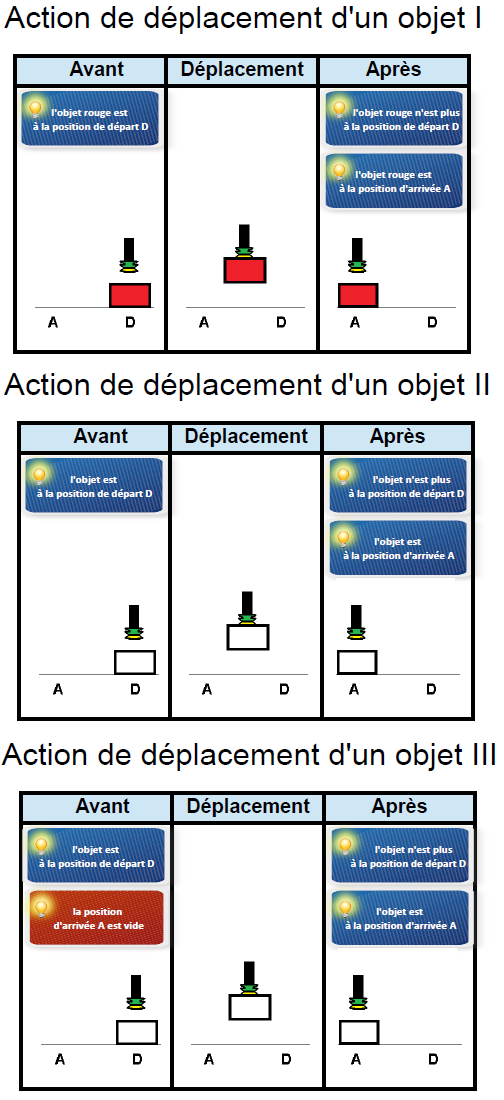
\includegraphics[scale=0.7]{figures/schema-all}
    \caption{Action model used in experiments}
    \label{fig:schema-all}
  \end{figure}
\newpage
%\section{Questionnaire}
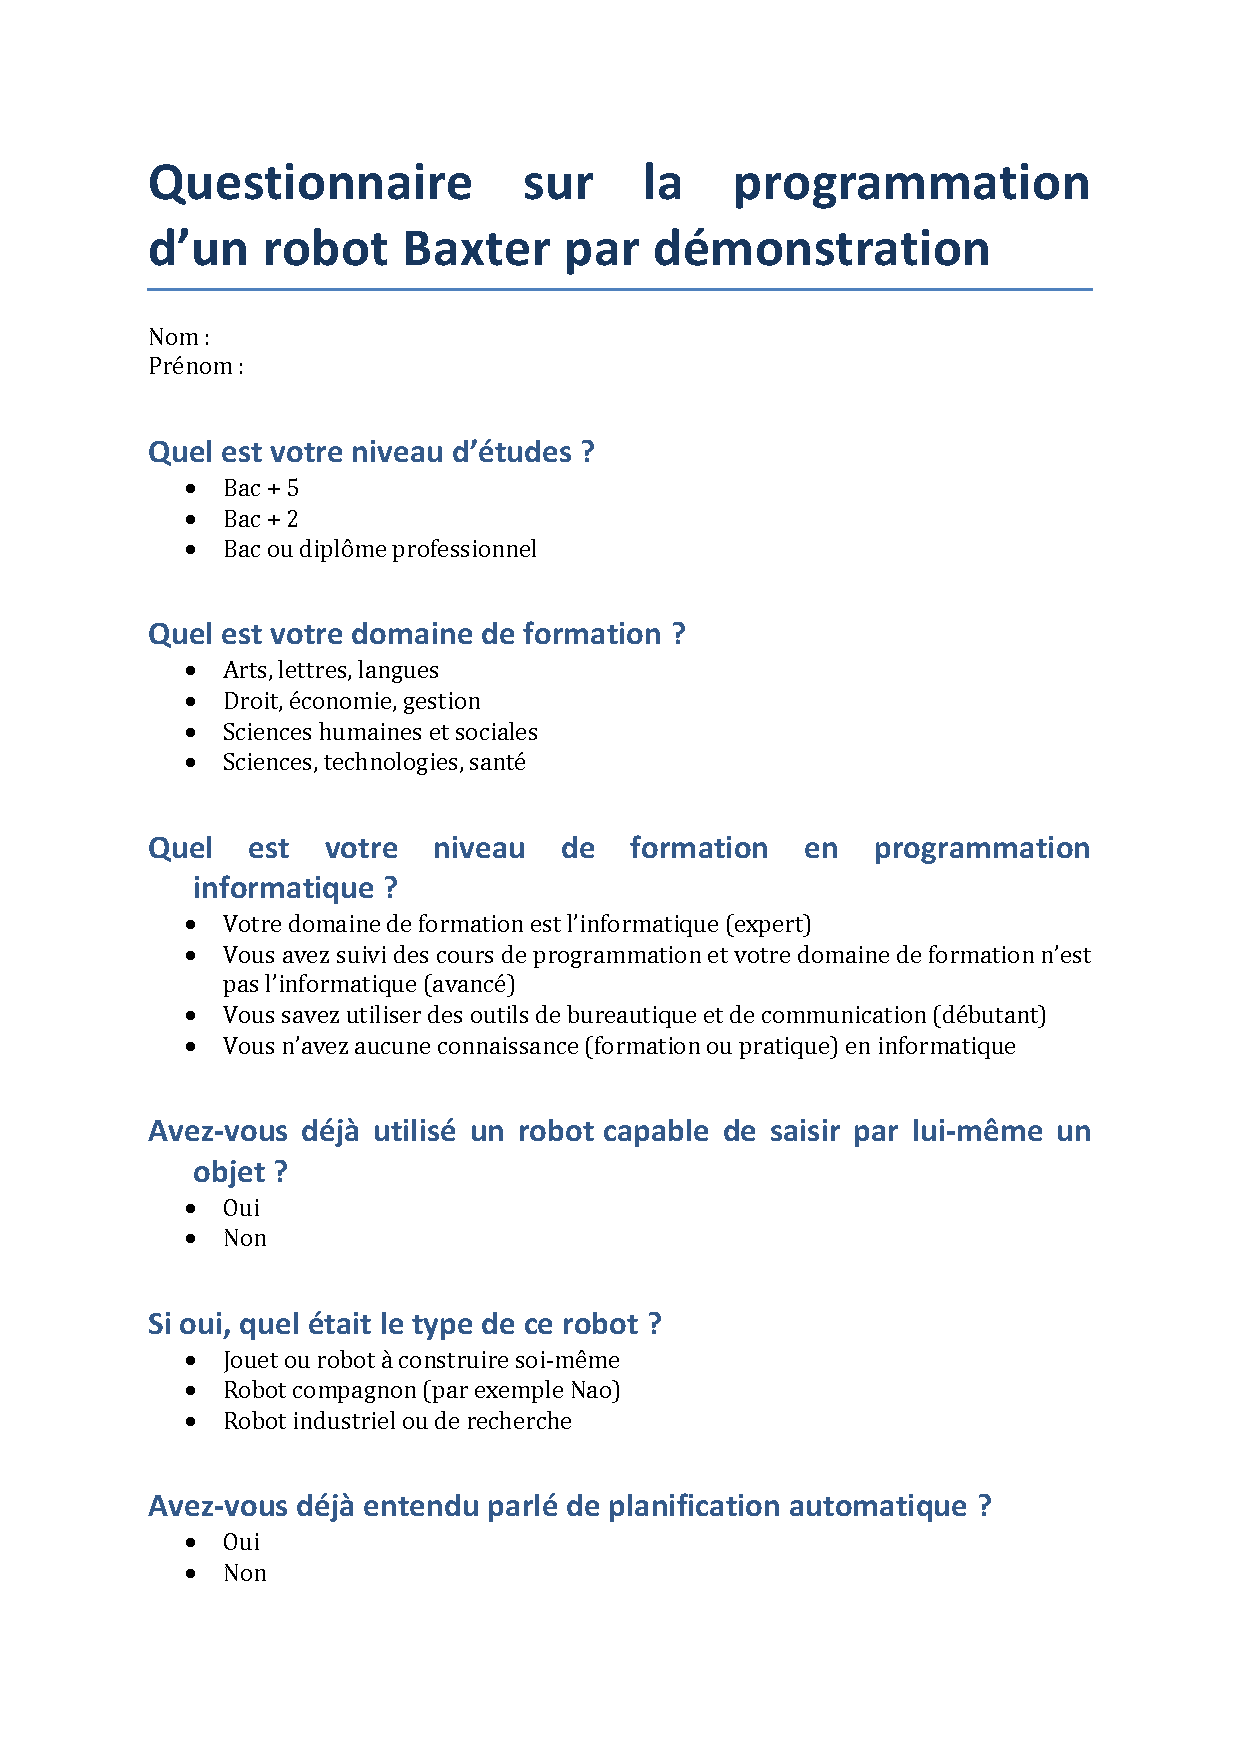
\includepdf[pages=1-3]{7-appendix/questionnaire.pdf}
%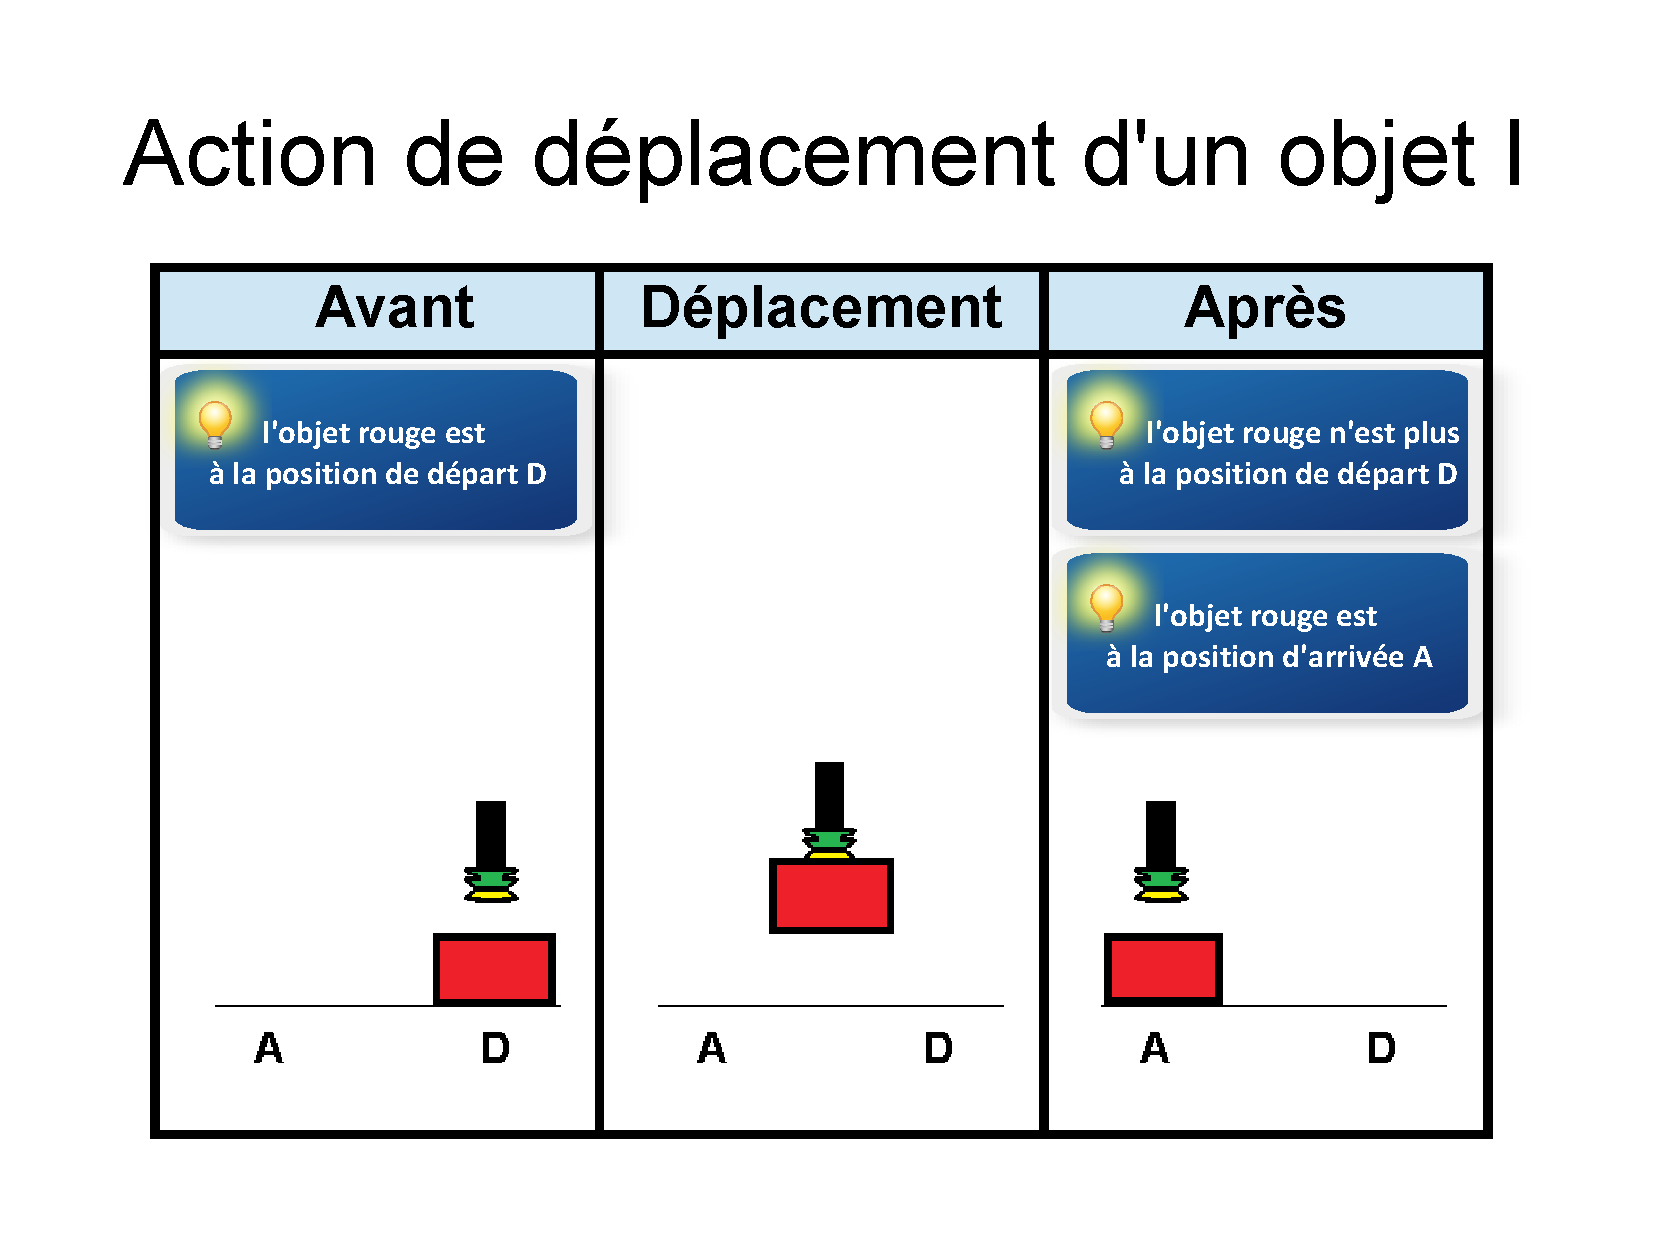
\includepdf[pages=1-3]{schema.pdf}
%\section{Experimental protocol}\label{protocol}
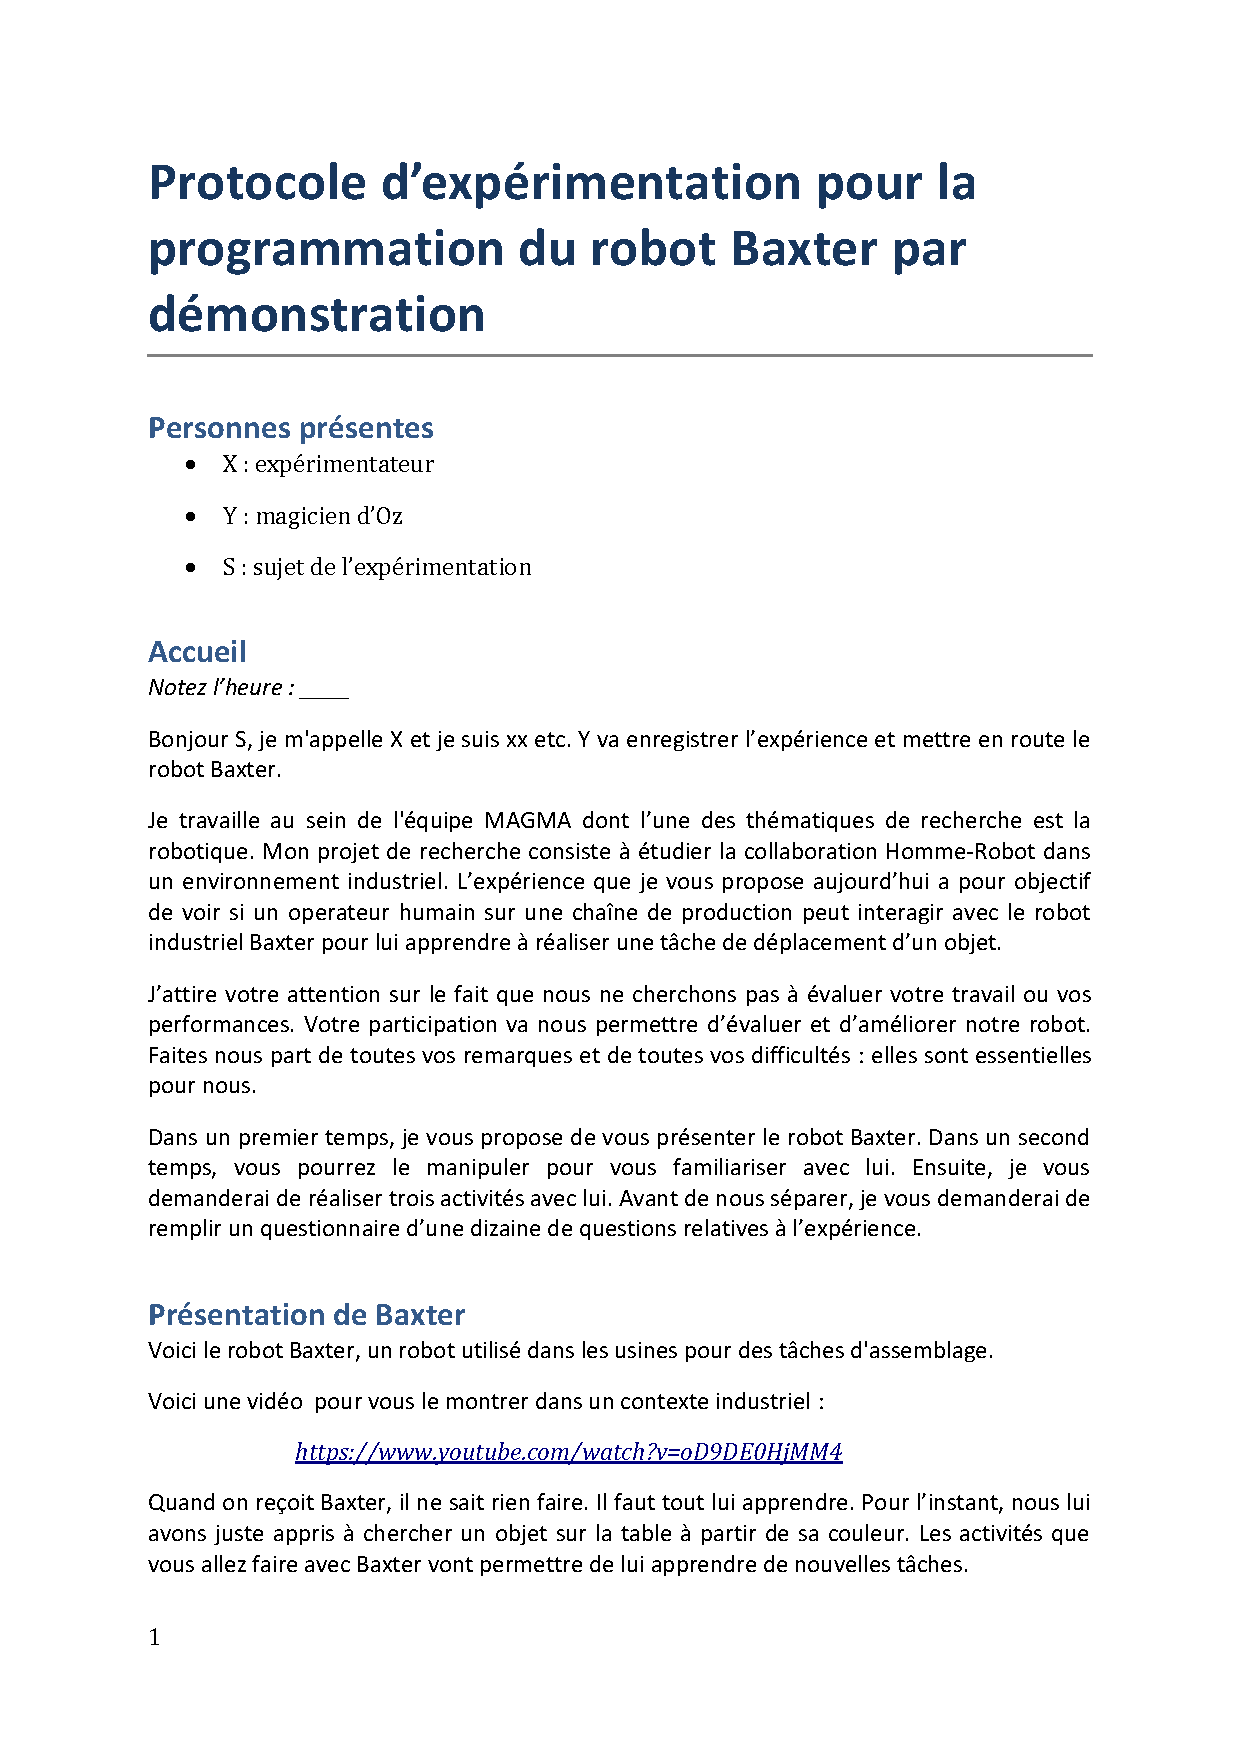
\includepdf[pages=1-7]{7-appendix/Protocole.pdf}
%\chapter{Notes during the experiments}
%\includepdf[pages=1-5]{notes.pdf}